\documentclass[11pt,a4paper]{article}

\usepackage[T1]{fontenc}
\usepackage[utf8]{inputenc}
\usepackage[english]{babel}
\usepackage[margin=2.3cm]{geometry}
\usepackage{amsmath,amssymb}
\usepackage{graphicx}
\usepackage{booktabs}
\usepackage{xcolor}
\usepackage[colorlinks=true,linkcolor=black,urlcolor=blue]{hyperref}
\usepackage{caption}
\usepackage{natbib}
\bibpunct{(}{)}{;}{a}{}{,}

\captionsetup{font=small,labelfont=bf}
\setlength{\parskip}{0.35em}

% This report is mostly tables, and with LaTeX's defaults they drifted two
% pages past the section that discusses them -- the convergence table ended up
% inside the Caveats. Loosen the float parameters so a page may be mostly
% float, and allow more than the default two per page.
\renewcommand{\topfraction}{0.92}
\renewcommand{\bottomfraction}{0.85}
\renewcommand{\textfraction}{0.06}
\renewcommand{\floatpagefraction}{0.72}
\setcounter{topnumber}{3}
\setcounter{bottomnumber}{2}
\setcounter{totalnumber}{4}
% ...and stop them crossing a section boundary, or the five figures all queue
% up behind the tables and come out after the bibliography.
\usepackage[section]{placeins}

\newcommand{\Msun}{M_\odot}
\newcommand{\Req}{R_{\mathrm{eq}}}
\newcommand{\Rpol}{R_{\mathrm{pol}}}
\newcommand{\Rvol}{R_{\mathrm{vol}}}
\newcommand{\Btor}{B_\varphi}
\newcommand{\Bpol}{B_{\mathrm{pol}}}
\newcommand{\Etor}{E_{\mathrm{tor}}}
\newcommand{\Epol}{E_{\mathrm{pol}}}
\newcommand{\Emag}{E_{\mathrm{mag}}}

\title{\textbf{Three-dimensional MHD evolution of an ultramassive white dwarf\\
with differential rotation and a mixed field}\\[0.3em]
\large Initial and final states at $192^3$ and $256^3$ --- interim report}
\author{Rafael C.\ R.\ de Lima}
\date{3 August 2026}

\begin{document}
\maketitle

\begin{abstract}
\noindent
A $2.005\,\Msun$ equilibrium with strong differential rotation and a
toroidal-dominated field, evolved in three-dimensional ideal MHD at two
resolutions. \textbf{The star survives and keeps its mass; its ordered field
does not.} At $192^3$, run to $t = 60$\,s, the magnetic energy falls by a
factor of $2170$ and the toroidal-to-poloidal amplitude ratio from $338$ to
$1.07$, while the mass stays within $0.3\%$. \textbf{The differential rotation
is not erased}: both grids hold
$\Omega_{\mathrm{out}}/\Omega_{\mathrm{core}}$ near $1/3$ throughout, nowhere
near the uniform rotation that would leave $2\,\Msun$ unsupported, and at
$t = 12$\,s they agree on it to $1.4\%$. The instability is $m=1$ and grows in
a few Alfv\'en times. Its rate is not converged --- it rises $47\%$ from
$192^3$ to $256^3$ --- and the post-saturation decay is not converged either,
in the opposite direction; the finer grid holds twice the magnetic energy at
$t = 12$\,s. \textbf{A further steepening of the differential rotation, seen at
$192^3$, does not survive refinement}: over $t = 12$ to $26.5$\,s the ratio
falls $8.2\%$ at $192^3$ and $1.0\%$ at $256^3$, and the redistribution of
$L_z$ between the inner and outer halves of the mass reverses sign. The total
angular momentum loss does converge, at $1.1\%$ against $1.2\%$ over the same
window. $256^3$ has reached $t = 26.5$\,s and is continuing.
\end{abstract}

%======================================================================
\section{Initial state}

\subsection{The star}

\begin{table}[h]
\centering\small
\begin{tabular}{llr}
\toprule
Mass & $M$ & $2.0052\,\Msun$ \\
 & $M/M_{\mathrm{Ch}}$ ($\mu_e = 2$) & $\mathbf{1.38}$ \\
Central density & $\rho_c$ & $3.00\times10^{9}$ g\,cm$^{-3}$ \\
Mean density & $\langle\rho\rangle$ & $3.30\times10^{7}$ g\,cm$^{-3}$ \\
Equatorial radius & $\Req$ & $3.917\times10^8$ cm \\
Polar radius & $\Rpol$ & $1.501\times10^8$ cm \\
Oblateness & $\Rpol/\Req$ & $\mathbf{0.383}$ \\
Volume-equivalent radius & $\Rvol$ & $3.07\times10^8$ cm \\
\midrule
Rotation law & $\Omega(\varpi) = \Omega_c A^2/(A^2+\varpi^2)$ & $A = 1.834\times10^8$ cm \\
Central angular velocity & $\Omega_c$ & $8.193$ rad\,s$^{-1}$ \quad ($P = 0.77$ s) \\
Equatorial angular velocity & $\Omega(\Req)$ & $1.47$ rad\,s$^{-1}$ \quad ($P = 4.3$ s) \\
Degree of differential rotation & $\Omega_c/\Omega(\Req)$ & $\mathbf{5.6}$ \\
Equatorial velocity & $v_{\mathrm{eq}}$ & $6.2\times10^3$ km\,s$^{-1}$ = $0.021\,c$ \\
Rotational support & $T/|W|$ & $0.0993$ \\
Mass shedding & $\Omega_{\mathrm{eq}}^2\Req/g_{\mathrm{eq}}$ & $0.469$ \\
\midrule
Dynamical time & $t_{\mathrm{dyn}}$ & $0.475$ s \\
Alfv\'en time & $t_A$ & $2.383$ s \\
Central rotation period & $P_{\mathrm{rot}}$ & $0.767$ s \\
\bottomrule
\end{tabular}
\caption{The configuration. It lies $38\%$ above the Chandrasekhar mass and can
only exist because of the differential rotation, which is also why it is so
flattened. It is not at breakup ($47\%$ of shedding) and is below both bar-mode
thresholds ($T/|W| = 0.099$ against $0.14$ secular and $0.27$ dynamical). The
surface period of $4.3$\,s is some three times shorter than the fastest white
dwarf spin claimed in the literature; this is a merger-remnant-like
configuration, not a model of an observed star.}
\end{table}

\subsection{The fields}

\begin{table}[h]
\centering\small
\begin{tabular}{lrrr}
\toprule
& analytic model & $192^3$ grid & $256^3$ grid \\
\midrule
$\max|\Btor|$ (G) & $3.231\times10^{13}$ & $3.196\times10^{13}$ & $3.204\times10^{13}$ \\
$\max|\Bpol|$ (G) & $7.63\times10^{9}$ & $9.46\times10^{10}$ & $8.41\times10^{10}$ \\
$\max|B|/B_c$ & $0.732$ & $0.724$ & $0.726$ \\
\midrule
$\Emag$ (erg) & $6.035\times10^{49}$ & $6.035\times10^{49}$ & $6.056\times10^{49}$ \\
$\Etor/\Emag$ & $0.99999995$ & $0.999997$ & $0.999998$ \\
$\Etor/\Epol$ & $\mathbf{2.18\times10^{7}}$ & $3.11\times10^{5}$ & $5.22\times10^{5}$ \\
$\max|\Btor|/\max|\Bpol|$ & $\mathbf{4234}$ & $338$ & $381$ \\
\midrule
$\Epol/|W|$ & $5.2\times10^{-10}$ & --- & --- \\
Toroidal filling factor & --- & $1.23\%$ & --- \\
\bottomrule
\end{tabular}
\caption{Mixed field, toroidal-dominated to one part in $10^7$ by energy: a
$10^9$\,G exterior dipole beside a $3\times10^{13}$\,G interior toroidal field.
The peak toroidal field is reconstructed on the grid to $98.9\%$ of the model
value at $192^3$; the poloidal component is not, because interpolating an
axisymmetric model onto a Cartesian mesh injects poloidal field an order of
magnitude above the true one. \emph{The poloidal quantities at $t=0$ are
therefore numerical floors, not physics}, and the growth measured later is
counted against them. The filling factor is
$8\pi\Etor/\max|\Btor|^2$ over the stellar volume.}
\end{table}

\subsection{Equation of state and method}

\begin{table}[h]
\centering\small
\begin{tabular}{ll}
\toprule
Equation of state & \texttt{ztwd}: zero-temperature degenerate electrons, $\mu_e = 2$ \\
 & \textbf{barotropic}, $P = P(\rho)$; all $\partial/\partial T$ vanish, $c_V = c_P = 0$ \\
Code & \textsc{Castro} 26.07 / AMReX; ideal MHD, constrained transport, HLLD \\
Grid & 3D Cartesian, single level, box $1.8\times10^9$ cm per side \\
 & $192^3$: $\mathrm{d}x = 9.375\times10^6$ cm \quad $256^3$: $7.031\times10^6$ cm \\
Gravity & \texttt{PoissonGrav}, full 3D solve (the quadrupole is large at $\Rpol/\Req = 0.38$) \\
Initial condition & Grad--Shafranov/SCF on $385\times769$ $(\varpi,z)$, interpolated from $\mathbf{A}$ \\
CFL & $0.5$ at $192^3$; $0.3$ at $256^3$ past $t \simeq 4.8$\,s \\
Floor / sponge & $\rho_{\min} = 10^2$ against ambient $2\times10^4$; sponge $10^4$--$10^5$ \\
Diagnostics & rebuilt from $B_x,B_y,B_z$; the native \texttt{emag\_density}, \\
 & \texttt{etor\_density} and \texttt{Div\_B} derives are corrupt (see Sec.~\ref{sec:caveats}) \\
\bottomrule
\end{tabular}
\end{table}

%======================================================================
\section{Final states}

\subsection{Same instant, both grids}

\begin{table}[h]
\centering\small
\begin{tabular}{lrrr}
\toprule
$t \simeq 5.2$\,s & $192^3$ & $256^3$ & ratio \\
\midrule
$\Etor$ (erg) & $1.965\times10^{49}$ & $1.784\times10^{49}$ & $0.91$ \\
$\Epol$ (erg) & $1.791\times10^{48}$ & $2.510\times10^{48}$ & $1.40$ \\
$\Emag/\Emag(0)$ & $35.5\%$ & $33.6\%$ & \\
$\Etor/\Epol$ & $11.0$ & $7.1$ & \\
$\max|\Btor|$ (G) & $4.539\times10^{13}$ & $4.045\times10^{13}$ & $0.89$ \\
$\max|\Bpol|$ (G) & $3.827\times10^{13}$ & $3.104\times10^{13}$ & $0.81$ \\
$\max|\Btor|/\max|\Bpol|$ & $1.19$ & $1.30$ & \\
$\max|B|/B_c$ & $1.118$ & $0.931$ & \\
$M$ ($\Msun$) & $2.0035$ & $2.0031$ & \\
$\Rvol$ ($10^8$ cm) & $3.51$ & $2.97$ & \\
\bottomrule
\end{tabular}
\caption{The two grids at the same physical time, at the end of the growth
phase. They agree on the state to within tens of percent, but not on the rate
that got there --- see Sec.~\ref{sec:conv}.}
\end{table}

\subsection{The common window, $t = 9$--$12$\,s}

The $256^3$ run has since reached its $12$\,s target, so the two grids can be
compared over a window rather than at an instant. That matters: the star
breathes by $\pm14\%$ every $1.498$\,s, and any single snapshot catches an
arbitrary phase of it. Table~\ref{tab:window} averages over the last two
periods, which removes the pulsation and leaves the state.

\begin{table}[h]
\centering\small
\begin{tabular}{lrrr}
\toprule
mean over $9$--$12$\,s & $192^3$ & $256^3$ & $256/192$ \\
\midrule
\multicolumn{4}{l}{\emph{The star --- converged}}\\
$M$ ($\Msun$) & $2.0028$ & $2.0042$ & $1.0007$ \\
$\Rvol$ ($10^8$ cm) & $3.113$ & $3.049$ & $0.98$ \\
$\Req$ ($10^8$ cm) & $3.895$ & $3.883$ & $\mathbf{1.003}$ \\
$\Rpol/\Req$ & $0.514$ & $0.501$ & $0.98$ \\
$V/V_0$ & $1.06$ & $0.99$ & $0.93$ \\
$\Omega_{\mathrm{core}}$ (rad\,s$^{-1}$) & $6.654$ & $6.733$ & $\mathbf{1.012}$ \\
$\Omega_{\mathrm{out}}$ (rad\,s$^{-1}$) & $2.294$ & $2.357$ & $\mathbf{1.027}$ \\
$\Omega_{\mathrm{out}}/\Omega_{\mathrm{core}}$ & $0.345$ & $0.350$ & $\mathbf{1.014}$ \\
$L_z$ ($10^{50}$ g cm$^2$ s$^{-1}$) & $2.168$ & $2.078$ & $0.96$ \\
$\max|B|/B_c$ & $0.771$ & $0.826$ & $1.07$ \\
\midrule
\multicolumn{4}{l}{\emph{Whole-star mass averages --- less well converged}}\\
$\bar\Omega$ (rad\,s$^{-1}$) & $3.992$ & $4.360$ & $1.09$ \\
$I = L_z/\bar\Omega$ ($10^{49}$ g cm$^2$) & $5.49$ & $4.78$ & $0.87$ \\
\midrule
\multicolumn{4}{l}{\emph{The field --- not converged}}\\
$\Etor$ (erg) & $4.07\times10^{48}$ & $8.00\times10^{48}$ & $\mathbf{1.96}$ \\
$\Epol$ (erg) & $3.07\times10^{47}$ & $8.24\times10^{47}$ & $\mathbf{2.69}$ \\
$\Emag/\Emag(0)$ & $7.3\%$ & $14.6\%$ & $2.01$ \\
$\Etor/\Epol$ & $13.3$ & $9.7$ & $0.73$ \\
$L_z^{\mathrm{outer}}/L_z^{\mathrm{inner}}$ & $5.04$ & $5.90$ & $1.17$ \\
\bottomrule
\end{tabular}
\caption{The two grids over the same three seconds, averaged over two
pulsation periods. The split is sharp and it is the main new result of this
report: everything about \emph{the star} agrees to a few percent --- mass,
size, shape, and above all the rotation, where the core, the outer shell and
their ratio all land within $3\%$ --- while everything about the \emph{energy}
in the field differs by a factor of two. The finer grid dissipates less, which
is exactly what an ideal-MHD run with no explicit resistivity should do.
The middle block is the honest exception: $\bar\Omega$ is mass-weighted over
the whole star, so it is set partly by the tenuous outer layers just above the
density cut, which are the least resolved part of the configuration. It
converges to $9\%$ rather than $1$--$3\%$, and $I = L_z/\bar\Omega$ inherits
that. The shell measurements are local and do not.}
\label{tab:window}
\end{table}

The rotation rows are the ones to take away. The conclusion that the star keeps
its differential rotation --- the property that lets it hold $2\,\Msun$ ---
was previously measured at one resolution only. It is now measured at two, and
they agree to $1.4\%$.

\subsection{Past $12$\,s: a test the fine grid fails}
\label{sec:latewindow}

The $256^3$ run has been continued and now reaches $t = 26.5$\,s, which puts a
second resolution on part of the late evolution as well. The comparison below
was fixed before the $256^3$ numbers were looked at: at $192^3$
$\Omega_{\mathrm{out}}/\Omega_{\mathrm{core}}$ falls $8.2\%$ over this window,
and anything between $6$ and $11\%$ at $256^3$ would have confirmed it.

\begin{table}[h]
\centering\small
\begin{tabular}{lrrl}
\toprule
$12$--$15$\,s $\to$ $23.5$--$26.6$\,s & $192^3$ & $256^3$ & verdict \\
\midrule
$L_z$ ($10^{50}$ g cm$^2$ s$^{-1}$) & $-1.1\%$ & $-1.2\%$ & converged \\
$\Omega_{\mathrm{out}}$ (rad\,s$^{-1}$) & $-4.9\%$ & $-4.4\%$ & converged \\
$M$ ($\Msun$) & $0.0\%$ & $0.0\%$ & converged \\
\midrule
$\Omega_{\mathrm{core}}$ (rad\,s$^{-1}$) & $\mathbf{+3.6\%}$ & $\mathbf{-3.4\%}$ & \textbf{opposite sign} \\
$\Omega_{\mathrm{out}}/\Omega_{\mathrm{core}}$ & $\mathbf{-8.2\%}$ & $\mathbf{-1.0\%}$ & \textbf{fails} \\
$L_z^{\mathrm{outer}}/L_z^{\mathrm{inner}}$ & $\mathbf{-3.7\%}$ & $\mathbf{+4.4\%}$ & \textbf{opposite sign} \\
\bottomrule
\end{tabular}
\caption{Means over two windows of two pulsation periods each, so the $\pm14\%$
breathing is averaged out rather than interpolated through. What the star loses
globally converges: the same $1.1$--$1.2\%$ of $L_z$, the same outer-shell
spin-down, the same flat mass. How it \emph{redistributes} that loss internally
does not. At $192^3$ the core spins up while the envelope slows, which reads as
angular momentum carried outward; at $256^3$ core and envelope slow together
and the profile keeps its shape.}
\label{tab:late}
\end{table}

\textbf{The steepening reported below at $192^3$ is therefore not a converged
result.} What survives refinement is the weaker and more important statement:
the ratio stays near $1/3$ on both grids and on neither does it climb towards
unity, so the differential rotation that holds $2\,\Msun$ is never removed. The
further claim --- that the field actively steepened the profile --- rests on a
core spin-up that reverses sign at $256^3$, and should be treated as a $192^3$
artefact until a third resolution says otherwise.

\subsection{The end state, $192^3$}

Only the $192^3$ run has reached a steady late state; it was carried to
$t = 60$\,s and stopped changing well before that.

\begin{table}[h]
\centering\small
\begin{tabular}{lrrr}
\toprule
$192^3$ & $t = 0$ & $t = 38.5$\,s & change \\
\midrule
\multicolumn{4}{l}{\emph{The star}}\\
$M$ ($\Msun$) & $2.00667$ & $2.00618$ & $\mathbf{-0.02\%}$ \\
$\Rvol$ ($10^8$ cm) & $3.068$ & $2.716$ & $-11\%$ \\
$\Req$ ($10^8$ cm) & $3.750$ & $3.204$ & $-15\%$ \\
$\Rpol/\Req$ & $0.425$ & $0.556$ & rounder \\
$\Omega_{\mathrm{core}}$ (rad\,s$^{-1}$)$^{\dagger}$ & $7.86$ & $7.59$ & $-3\%$ \\
$\Omega_{\mathrm{out}}$ (rad\,s$^{-1}$)$^{\dagger}$ & $2.56$ & $1.92$ & $-25\%$ \\
$\Omega_{\mathrm{out}}/\Omega_{\mathrm{core}}$$^{\dagger\ddagger}$ & $0.341$ & $0.266$ & $-22\%$ \\
$L_z$ ($10^{50}$ g cm$^2$ s$^{-1}$)$^{\dagger}$ & $1.979$ & $2.101$ & $-5.5\%$ from peak \\
$L_z^{\mathrm{outer}}/L_z^{\mathrm{inner}}$$^{\dagger\ddagger}$ & $6.35$ & $4.35$ & $-32\%$ \\
$I$ ($10^{49}$ g cm$^2$)$^{\dagger}$ & $4.16$ & $4.59$ & $-8.8\%$ from $t=12$ \\
\midrule
\multicolumn{4}{l}{\emph{The field}}\\
$\Emag$ (erg) & $6.035\times10^{49}$ & $2.782\times10^{46}$ & $\mathbf{/\,2170}$ \\
$\Etor$ (erg) & $6.035\times10^{49}$ & $2.658\times10^{46}$ & $/\,2270$ \\
$\Epol$ (erg) & $1.942\times10^{44}$ & $1.236\times10^{45}$ & $\times 6.4$ \\
$\Etor/\Epol$ & $3.11\times10^{5}$ & $21.5$ & $/\,1.4\times10^{4}$ \\
$\max|\Btor|$ (G) & $3.196\times10^{13}$ & $1.227\times10^{12}$ & $/\,26$ \\
$\max|\Bpol|$ (G) & $9.46\times10^{10}$ & $1.148\times10^{12}$ & $\times 12$ \\
$\max|\Btor|/\max|\Bpol|$ & $\mathbf{338}$ & $\mathbf{1.07}$ & $/\,316$ \\
$\max|B|/B_c$ & $0.724$ & $0.031$ & \\
\bottomrule
\end{tabular}
\caption{Initial and end state at $192^3$. The star keeps its mass to $0.02\%$;
the field is reduced by three orders of magnitude in energy and ends with its
two components equal in peak strength. $^{\dagger}$Rotation and $L_z$ are
quoted at $t = 60$\,s, the end of the run; the field and shape columns at
$t = 38.5$\,s, the last instant processed with the field diagnostics.
$^{\ddagger}$\textbf{Not converged.} These two rows measure how the star
redistributes angular momentum internally, and over the window where the
$256^3$ run also exists they change by $-1.0\%$ and $+4.4\%$ there against
$-8.2\%$ and $-3.7\%$ here (Table~\ref{tab:late}). The rows are kept because
they are what this run does; they are not evidence about the star.}
\label{tab:end}
\end{table}

Three points in Table~\ref{tab:end} carry most of the physics.

\paragraph{The mass does not move.} $0.02\%$ from start to end, $0.3\%$ in
amplitude along the way, while the magnetic energy of the same star falls by a
factor of $2170$. Whatever destroys the field does not unbind the star.

\paragraph{Losing $L_z$ and spinning up is expected here.} $L_z = I\bar\Omega$
and $I$ is not constant: between $t = 12$ and $60$\,s the star loses $2.8\%$ of
its angular momentum, contracts enough to lose $8.8\%$ of its moment of
inertia, and gains $6.6\%$ in $\bar\Omega$ (Fig.~\ref{fig:rot}b). This is not
an oddity of the simulation. It is the behaviour known for rotating white
dwarfs near the maximum mass, where a configuration shedding angular momentum
contracts and spins up rather than spinning down --- the spin-up branch
discussed by \citet{boshkayev2013}. Their analysis is uniformly rotating and
general relativistic while this configuration is differentially rotating,
Newtonian and magnetised, so the correspondence is in the mechanism and not in
the numbers.

\paragraph{The differential rotation survives; that it \emph{strengthens} is
$192^3$ only.} Everything in this paragraph is measured on the coarse grid, and
Table~\ref{tab:late} shows that the part about steepening does not survive
refinement --- read it as what the $192^3$ run says, not as a result.
Fig.~\ref{fig:rot} is the diagnostic the long run was extended to provide. The
magnetic transport is real and its signature is unambiguous: $L_z$ falls at
$0.21\%$\,s$^{-1}$ while the toroidal field lives and $0.10\%$\,s$^{-1}$ after it
is gone. With no explicit viscosity and no explicit resistivity in these runs,
nothing else in the scheme brakes anything, so that factor of two identifies
the agent.

But the transport does not homogenise the star. Had it done so,
$\Omega_{\mathrm{out}}/\Omega_{\mathrm{core}}$ would climb towards unity; it
falls instead, from $0.34$ to $0.27$. The core holds its angular velocity to
$3\%$ over $60$\,s while the outer shell loses $25\%$ of its own --- angular
momentum is carried outward and out of the star, and it is the outer layers
that pay. Split by mass rather than by radius the same thing shows:
$L_z^{\mathrm{outer}}/L_z^{\mathrm{inner}}$ falls from $6.35$ to $4.35$,
because the outer half of the mass loses $1\%$ of its angular momentum while
the star as a whole loses $5.5\%$ and the inner half gains.

\emph{The star survives because the field never came close to removing what
supports it} --- and that half of the sentence is converged. The other half,
that the field steepened the profile rather than flattening it, is not: over
$t = 12$ to $26.5$\,s the $256^3$ run loses $1.0\%$ of the ratio against
$8.2\%$ here, its core slows instead of speeding up, and its
$L_z^{\mathrm{outer}}/L_z^{\mathrm{inner}}$ moves the other way
(Table~\ref{tab:late}). The global losses agree between the grids; only their
internal redistribution does not, which points at the coarse grid's own
transport rather than at the field.

\paragraph{``Destroyed'' means disordered, not weakened --- until late.} At
$t = 5.2$\,s the peak toroidal field is \emph{higher} than initially,
$4.54\times10^{13}$ against $3.20\times10^{13}$\,G, while the energy has fallen
by a factor of three: the field is concentrating into filaments, its effective
volume dropping from $1.49\times10^{24}$ to $2.40\times10^{23}$\,cm$^3$. Only
afterwards does the peak collapse as well, to $1.23\times10^{12}$\,G.

\begin{figure}[t]
\centering
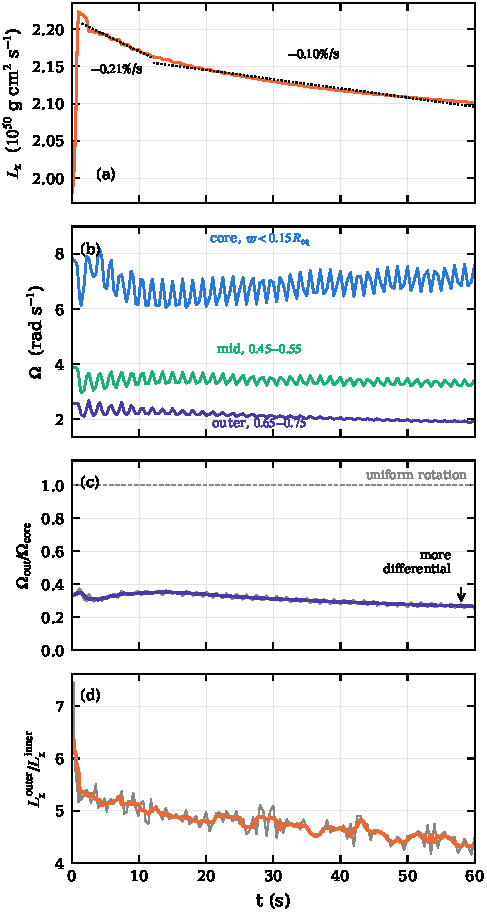
\includegraphics[width=0.60\textwidth]{figures/rotation_192.pdf}
\caption{$192^3$ over the full $60$\,s. \textbf{(a)} $L_z$ of the star, with
the two braking rates fitted; the $12\%$ rise in the first second is the
initial transient settling. \textbf{(b)} the decomposition $L_z = I\bar\Omega$,
normalised at $t = 12$\,s, which answers the obvious objection to (a): the star
loses angular momentum and its angular velocity rises anyway, because $I$ is
not constant. Between $t = 12$ and $60$\,s, $L_z$ falls $2.8\%$, $I$ falls
$8.8\%$ as the star contracts, and $\bar\Omega = L_z/I$ gains $6.6\%$ --- a
skater, minus the losses. \textbf{(c)} $\Omega$ mass-weighted in three
cylindrical shells, all chosen to stay inside the star at every phase of the
$1.5$\,s pulsation --- note they sit at fixed fractions of the \emph{initial}
$\Req$, so part of the decline in the outer one is the star having shrunk out
from under it. \textbf{(d)} the differential rotation; uniform rotation would
be $1$ and the star moves away from it. \textbf{(e)} $L_z$ of
the outer half of the \emph{mass} over that of the inner half --- split by
mass rather than radius, with the dividing radius recomputed at every snapshot,
because a shell at fixed $\varpi$ would measure the pulsation instead of the
transport. In (c) and (d) a running mean over one pulsation period is drawn
over the raw curve; the ripple is the pulsation and aliases badly against
coarse sampling.}
\label{fig:rot}
\end{figure}

%======================================================================
\section{The evolution between them}

\begin{figure}[t]
\centering
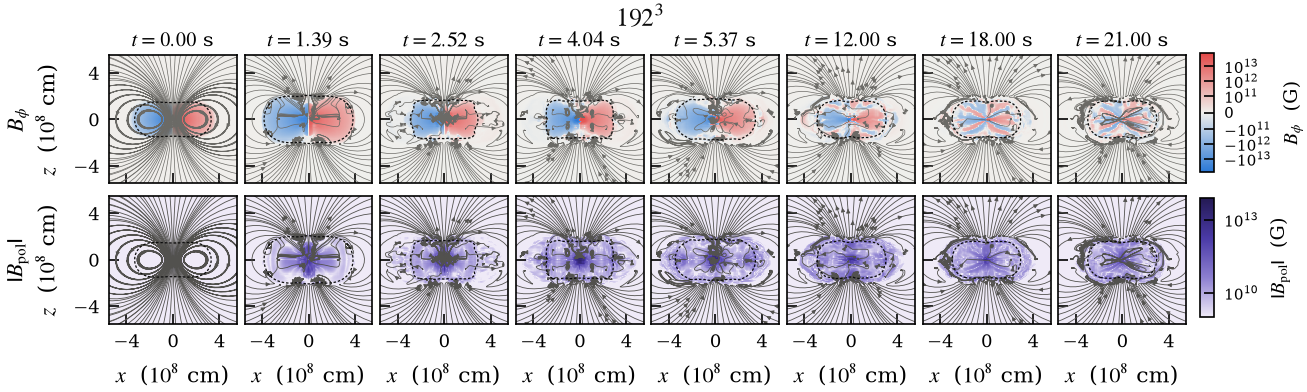
\includegraphics[width=\textwidth]{figures/field_sequence_192.png}
\caption{$192^3$. \textbf{Top:} equatorial cut $z=0$, where $\Btor$ lies in the
plane, so the streamlines \emph{are} the toroidal field lines --- circles while
the star is axisymmetric. \textbf{Bottom:} meridional cut $y=0$, where the
in-plane field \emph{is} the poloidal one. Colour is $\Btor$ and $|\Bpol|$
respectively, both starting at $10^{10}$\,G so the two rows are comparable; the
near-empty poloidal panel at $t=0$ is the statement that the poloidal field is
three decades below the toroidal one. Same scales as Fig.~\ref{fig:seq256}.}
\label{fig:seq192}
\end{figure}

The field goes through three phases, all visible in Fig.~\ref{fig:seq192}.

\begin{table}[h]
\centering\small
\begin{tabular}{llll}
\toprule
Phase & Window & Rate & Signature \\
\midrule
Growth & $t = 1.3$--$4.0$\,s & $\sigma = 1.369$ s$^{-1}$ ($r=0.994$) & $\Epol$ exponential; \\
& & $e$-fold of amplitude $0.61\,t_A$ & $m=1$ takes over \\
Saturation & $t \simeq 5.3$\,s & --- & $\Epol$ peaks at $10^4\times$ its floor; \\
& & & $\max\Btor/\max\Bpol \to 1.19$ \\
Decay & $t = 5.4$--$30$\,s & $e$-fold $3.6$--$4.0$\,s & $\Etor$ falls $10^3$ \\
Residual & $t > 30$\,s & $e$-fold $37$\,s & $\Emag \simeq 3\times10^{46}$ erg, flat \\
\bottomrule
\end{tabular}
\caption{Phases of the field evolution at $192^3$. The decay stalls after
$t \simeq 30$\,s: the field does not go to zero but settles at a disordered
residual of order $10^{12}$\,G.}
\end{table}

\paragraph{The mode is $m=1$.} An azimuthal Fourier projection gives
$|m{=}1|/|m{=}0| = 1.2\times10^{-16}$ at $t=0$ --- the initial condition is
axisymmetric to machine precision. From $t \simeq 2.5$\,s the poloidal field is
$m=1$ dominated, with $|B_{z,m=1}|/|B_{z,m=0}|$ reaching $21$ at $t=4$\,s, and
the toroidal $m=1$ saturates at $\simeq 10\%$ of the axisymmetric component.
This rules out the axisymmetric MRI, which could not exist here in any case:
built from the \emph{vertical} field, $\lambda_{\mathrm{MRI}} = 2.9\times10^4$\,cm,
or $0.003$ of a cell. What remains is the Tayler kink or the non-axisymmetric
toroidal-field MRI, which the mode number alone cannot separate.

\paragraph{The star pulsates and does not stop.} Past the initial transient,
$\rho_{\max}$ settles into a clean periodic oscillation of period $1.498$\,s
($3.15\,t_{\mathrm{dyn}}$, $1.95$ rotations) at $\pm14.4\%$, with an envelope
$e$-folding near $140$\,s. It is still running at $t=60$\,s.

\begin{figure}[t]
\centering
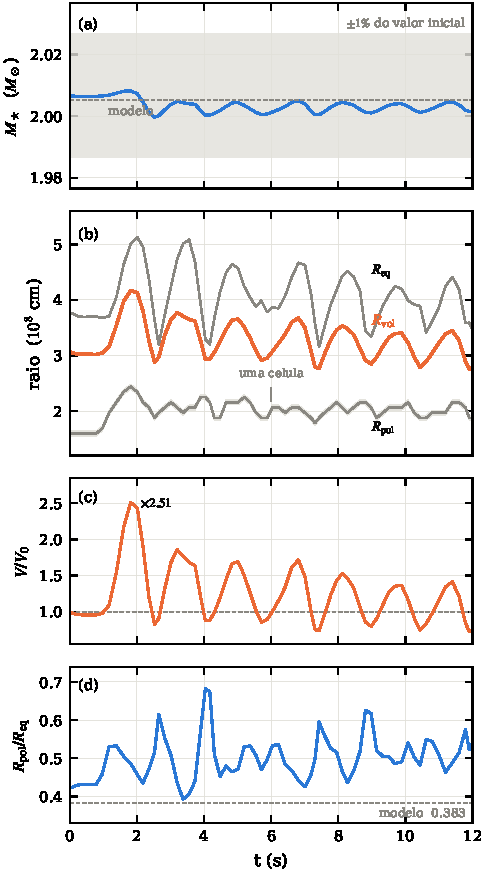
\includegraphics[width=0.49\textwidth]{figures/mass_radius_192.pdf}
\hfill
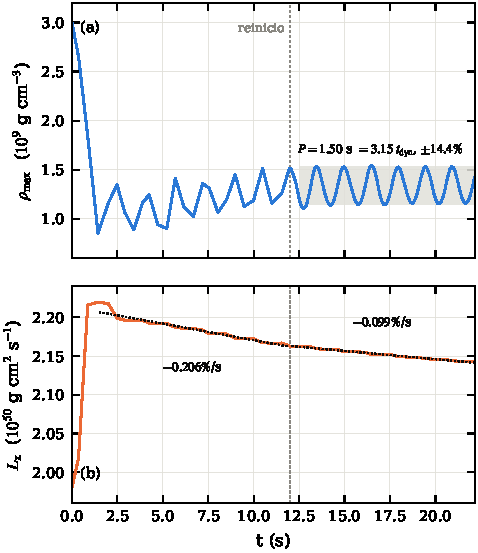
\includegraphics[width=0.49\textwidth]{figures/long_run_192.pdf}
\caption{\textbf{Left, $192^3$ to $t=12$\,s:} mass against a $\pm1\%$ band; the
three radii with one grid cell drawn around $\Rpol$; volume; oblateness.
\textbf{Right, to $t=22$\,s:} central density, and axial angular momentum with
the two braking rates fitted. The dashed vertical is the restart at $t=12$\,s.}
\end{figure}

%======================================================================
\section{Numerical convergence}
\label{sec:conv}

\begin{table}[h]
\centering\small
\begin{tabular}{lccl}
\toprule
& $192^3$ & $256^3$ & verdict \\
\midrule
Mass range ($\Msun$) & $1.9997$--$2.0082$ & $2.0021$--$2.0073$ & converged \\
$\Rvol(t=0)$ ($10^8$ cm) & $3.068$ & $3.069$ & converged ($0.03\%$) \\
$\Omega_{\mathrm{core}}$, $9$--$12$\,s (rad\,s$^{-1}$) & $6.654$ & $6.733$ & converged ($1.2\%$) \\
$\Omega_{\mathrm{out}}/\Omega_{\mathrm{core}}$, $9$--$12$\,s & $0.345$ & $0.350$ & \textbf{converged ($1.4\%$)} \\
$\max|B|$, $9$--$12$\,s (G) & $3.40\times10^{13}$ & $3.65\times10^{13}$ & converged ($7\%$) \\
\midrule
$\sigma$ from $\Epol$ (s$^{-1}$) & $1.369$ & $2.007$ & \textbf{$+47\%$, not converged} \\
$\sigma$ from the $m=1$ mode (s$^{-1}$) & $1.968$ & $2.752$ & $+40\%$, same factor \\
$\Epol(t=0)$, the floor (erg) & $1.94\times10^{44}$ & $1.16\times10^{44}$ & finer seed is smaller \\
$\min(\max\Btor/\max\Bpol)$ & $1.19$ & $\mathbf{0.805}$ & instability goes further \\
\quad at $t = 12$\,s & $2.93$ & $\mathbf{1.06}$ & fine grid $\sim3\times$ further along \\
\midrule
Decay rate $\gamma$ of $\Etor$, $6$--$12$\,s & $0.282$\,s$^{-1}$ & $0.141$\,s$^{-1}$ & \textbf{$/\,2.0$, not converged} \\
\quad as an $e$-folding & $3.5$\,s & $7.1$\,s & \\
$\Emag$ at $t = 12$\,s (erg) & $4.4\times10^{48}$ & $8.8\times10^{48}$ & $\times2.0$ \\
First volume peak & $2.51\,V_0$ & $1.79\,V_0$ & early pulsation is numerical \\
\bottomrule
\end{tabular}
\caption{Three verdicts. \emph{Converged:} everything about the star --- mass,
size, peak field, and the whole rotation profile. \emph{Not converged:} the
growth rate rises with resolution while the decay rate falls, each by about a
factor of two per refinement, so the measured growth is a lower bound and the
measured decay an upper bound; the coarse grid exaggerates the violence at both
ends. The early large-amplitude pulsation is largely the initial condition
ringing on the mesh.}
\end{table}

\begin{figure}[t]
\centering
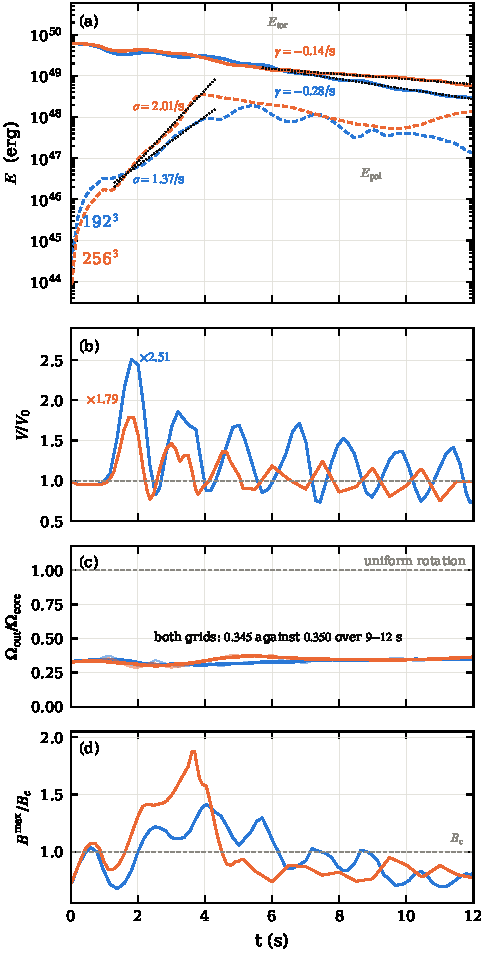
\includegraphics[width=0.66\textwidth]{figures/convergence_192_256.pdf}
\caption{$192^3$ against $256^3$ over the full $12$\,s. \textbf{(a)} Toroidal
(solid) and poloidal (dashed) energy, with the fitted growth $\sigma$ and decay
$\gamma$. The two rates move in \emph{opposite} directions with refinement.
\textbf{(b)} $V/V_0$: the first peak drops from $2.51$ to $1.79$, its excess
over unity scaling as $\mathrm{d}x^{2.3}$. \textbf{(c)} The differential
rotation --- neither grid approaches uniform rotation and the two agree to
$1.4\%$. \textbf{(d)} Peak field against $B_c$; above the Landau field for
roughly half the run at both resolutions.}
\label{fig:conv}
\end{figure}

\begin{figure}[t]
\centering
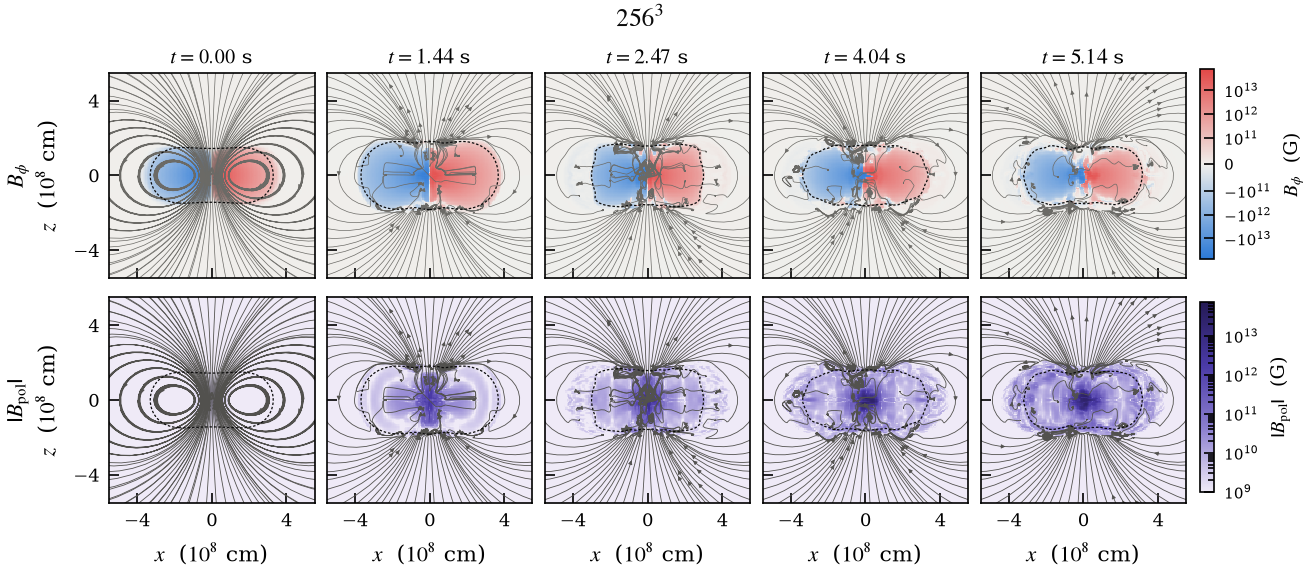
\includegraphics[width=\textwidth]{figures/field_sequence_256.png}
\caption{$256^3$, same layout, planes and colour scales as
Fig.~\ref{fig:seq192}.}
\label{fig:seq256}
\end{figure}

One row deserves reading twice. The amplitude ratio $\max\Btor/\max\Bpol$ dips
below unity only at $256^3$ --- the poloidal field overtakes the toroidal in
peak strength there and never does at $192^3$ --- and at $t = 12$\,s it stands
at $1.06$ on the fine grid against $2.93$ on the coarse. The $192^3$ run does
not reach $1.07$ until $t = 38.5$\,s (Table~\ref{tab:end}). In terms of field
topology the fine grid at $12$\,s is where the coarse grid is at nearly
$40$\,s: refinement does not merely sharpen the picture, it advances the
evolution. That is one more reason to treat every rate quoted here as a bound.

There is no explicit resistivity in these runs, so the decay of $\Etor$
\emph{is} the numerical resistivity, and the two grids measure it. Halving
$\gamma$ while $\mathrm{d}x$ falls by a factor $1.33$ puts it at
$\mathrm{d}x^{2.4}$, consistent with the second-order scheme and extrapolating
to zero. Read literally, that says the field decay seen here is a resolution
artefact and the physical star would keep its field far longer --- but a
two-point fit cannot distinguish that from a decay that converges to something
small but finite, and the growth rate moving the other way ($\mathrm{d}x^{-1.3}$)
warns that both ends of the evolution are still mesh-limited.

Settling the rate would need $384^3$, about five times the cost of $256^3$. The
alternative, and probably the right one, is explicit resistivity, giving the
problem a physical dissipation scale instead of letting the mesh set it;
\textsc{Castro} does not currently implement it.

%======================================================================
\section{Caveats}
\label{sec:caveats}

\begin{enumerate}\itemsep2pt
\item \textbf{The EOS is barotropic.} \texttt{ztwd} has no thermal reservoir, so
      the $6\times10^{49}$\,erg that leave the field have no physical
      destination and are dissipated at the grid scale. We can say the ordered
      field is destroyed; we cannot say where the energy went. The
      stratification is also neutral, with no buoyancy to limit the mode --- in
      a stratified star the rate would be lower, making $\sigma$ a
      \emph{physical} upper bound while it is a \emph{numerical} lower bound.
\item \textbf{Part of the run is outside the EOS validity range.} $\max|B|$
      reaches $1.41\,B_c$ at $t = 4.0$\,s at $192^3$ and $1.88\,B_c$ at
      $t = 3.6$\,s at $256^3$, exceeding the Landau critical field in $44\%$ and
      $48\%$ of the sampled instants respectively. This does \emph{not} improve
      with resolution --- the finer grid goes further above $B_c$, not less far.
      The late state, at $0.03\,B_c$, is well inside.
\item \textbf{The poloidal field at $t=0$ is a numerical floor.} Cartesian
      interpolation of an axisymmetric model injects $\Epol$ some $70$ times
      above the model's value even at $256^3$. All poloidal growth is measured
      against that floor, which is why it is quoted alongside.
\item \textbf{The internal redistribution of $L_z$ is not converged, and one
      claim has already fallen to it.} The two grids overlap to $t = 26.5$\,s
      and agree on what the star loses --- $1.1\%$ against $1.2\%$ of $L_z$,
      the same outer-shell spin-down --- but not on where it goes. The $192^3$
      core spins up and the profile steepens; the $256^3$ core slows and the
      profile holds its shape (Sec.~\ref{sec:latewindow}). Since there is no
      explicit viscosity or resistivity, the transport in both runs is whatever
      the scheme supplies, and the coarse grid supplies more of it. Anything
      here that depends on \emph{internal} redistribution --- the steepening,
      $L_z^{\mathrm{outer}}/L_z^{\mathrm{inner}}$, and by extension the
      $L_z = I\bar\Omega$ spin-up, which is built on the same shells --- should
      be read as $192^3$ behaviour pending a third resolution.
\item \textbf{Beyond $26.5$\,s only $192^3$ exists.} The settled $1.50$\,s
      pulsation and the halving of the braking rate once the field is gone are
      measured on one grid. The $256^3$ continuation towards $60$\,s is
      running.
\item \textbf{Native magnetic diagnostics are unusable.} \texttt{emag\_density},
      \texttt{etor\_density} and \texttt{Div\_B} pack face-centred components of
      different index types into one cell-centred FAB and read past the end of
      the box, \texttt{Div\_B} reaching $3\times10^{146}$ where it should be
      $\sim0$. Everything here is rebuilt from $B_x,B_y,B_z$, which are correct.
\end{enumerate}

%======================================================================
\section*{Status}

$192^3$: complete, $t = 60$\,s. \quad
$256^3$: running, $t = 30.5$\,s of a $60$\,s target; diagnostics processed to
$t = 26.5$\,s.

Inputs, submission scripts, diagnostic tools, data and figure code are under
version control in the \texttt{WD\_MAG} repository.

\begin{thebibliography}{9}
\bibitem[Boshkayev et al.(2013)]{boshkayev2013}
Boshkayev, K., Rueda, J.~A., Ruffini, R., \& Siutsou, I. 2013,
\textit{On General Relativistic Uniformly Rotating White Dwarfs},
ApJ, 762, 117.
\end{thebibliography}

\end{document}
